\documentclass[11pt]{article}
\usepackage[T1]{fontenc}
\usepackage{lmodern}
\input{glyphtounicode}
\input{glyphtounicode-cmex}
\pdfgentounicode=1
\pdfglyphtounicode{negationslash}{0338}
\usepackage[margin=1in]{geometry}
\usepackage{amsmath,amssymb,amsthm,mathtools}
\usepackage{microtype,booktabs,enumitem,needspace,tikz}
\usetikzlibrary{arrows.meta,positioning,calc}
\usepackage[colorlinks=true,linkcolor=blue!45!black,citecolor=blue!45!black,urlcolor=blue!45!black]{hyperref}
\usepackage[capitalise,noabbrev]{cleveref}
\ifdefined\pdfinfoomitdate\pdfinfoomitdate=1\fi
\ifdefined\pdftrailerid\pdftrailerid{}\fi
\ifdefined\pdfsuppressptexinfo\pdfsuppressptexinfo=15\fi
\newtheorem{theorem}{Theorem}[section]
\newtheorem{lemma}[theorem]{Lemma}
\newtheorem{proposition}[theorem]{Proposition}
\newtheorem{corollary}[theorem]{Corollary}
\theoremstyle{definition}
\newtheorem{definition}[theorem]{Definition}
\theoremstyle{remark}
\newtheorem{remark}[theorem]{Remark}
\newtheorem{example}[theorem]{Example}
\newcommand{\R}{\mathbb R}
\newcommand{\N}{\mathbb N}
\newcommand{\Z}{\mathbb Z}
\newcommand{\E}{\mathbb E}
\renewcommand{\P}{\mathbb P}
\DeclareMathOperator{\supp}{supp}
\DeclareMathOperator{\Law}{Law}
\DeclareMathOperator{\Var}{Var}
\DeclareMathOperator{\dist}{dist}
\newcommand{\eps}{\varepsilon}
\numberwithin{equation}{section}
\setlength{\emergencystretch}{2em}
\setlist{topsep=4pt,itemsep=3pt,parsep=0pt}
\title{The entropy-rate dimension formula for self-similar measures on the line}
\author{OpenAI}
\date{September 24, 2026}
\hypersetup{pdftitle={The entropy-rate dimension formula for self-similar measures on the line},pdfauthor={OpenAI}}
\begin{document}
\maketitle
\begin{abstract}
We prove that the Hausdorff dimension of every finite real self-similar
measure equals the minimum of one and its random-walk entropy rate divided
by its Lyapunov exponent. Exact overlaps are allowed, and the contraction
ratios may be unequal and negative. This resolves the entropy-rate dimension
conjecture.
\end{abstract}
\tableofcontents
\section{Introduction}\label{sec:introduction}

Let $\Lambda$ be a finite nonempty alphabet, and let
\[
 \Phi=(\varphi_i)_{i\in\Lambda},\qquad
 \varphi_i(x)=r_i x+t_i,\qquad t_i\in\R,\quad 0<|r_i|<1.
\]
The family is indexed: different symbols may specify the same map.
Given a probability vector $p=(p_i)_{i\in\Lambda}$ with $p_i>0$, its
self-similar measure is the unique Borel probability measure satisfying
\[
 \mu=\sum_{i\in\Lambda}p_i(\varphi_i)_*\mu.
\]
Equivalently, $\mu$ is the law of
$\lim_{n\to\infty}\varphi_{I_1}\circ\cdots\circ\varphi_{I_n}(0)$,
where the symbols $I_j$ are independent with law $p$.
The limit exists uniformly in the address: if
$r_{\max}=\max_i|r_i|$ and $T_0=\max_i|t_i|$, all coding limits
have absolute value at most $T_0/(1-r_{\max})$.

For a word $w=i_1\cdots i_n$, write
$\varphi_w=\varphi_{i_1}\circ\cdots\circ\varphi_{i_n}$ and
$p_w=p_{i_1}\cdots p_{i_n}$.  An \emph{exact overlap} is an equality
$\varphi_u=\varphi_v$ for distinct words of the same positive length.
Equality here means equality of the complete affine maps, including
both the signed slope and the translation.  We allow all such overlaps.

The relevant entropy counts maps rather than addresses.  Set
\[
 G_n=\varphi_{I_1}\circ\cdots\circ\varphi_{I_n},\qquad
 \P(G_n=g)=\sum_{w\in\Lambda^n:\,\varphi_w=g}p_w.
\]
All logarithms below have base two.  For a finite-valued random variable
$Z$, its Shannon entropy is $H(Z)=-\sum_z\P(Z=z)\log\P(Z=z)$,
with $0\log0=0$.  Define the random-walk entropy rate and the Lyapunov
exponent by
\begin{equation}\label{eq:rate-and-lyapunov}
 h=h_{\mathrm{RW}}(\Phi,p)
   :=\lim_{n\to\infty}\frac{H(G_n)}n
    =\inf_{n\ge1}\frac{H(G_n)}n,
 \qquad
 \chi=-\sum_i p_i\log|r_i|>0.
\end{equation}
Indeed, a length-$(n+m)$ map is a function of two independent maps
with laws $G_n,G_m$, so $H(G_{n+m})\le H(G_n)+H(G_m)$; subadditivity
gives the displayed limit and infimum.  Also
$0\le h\le H(p):=-\sum_i p_i\log p_i$.  The ratio $h/\chi$ is
independent of the common logarithm base.

We use the lower Hausdorff dimension of a measure:
\[
 \dim_H\nu=\inf\{\dim_H E:E\subset\R\text{ Borel},\ \nu(E)>0\}.
\]
Feng--Hu's exact-dimensionality theorem
\cite[Theorem~2.8]{FengHu2009} applies to finite self-similar systems
without separation.  Indeed, the maps preserve a sufficiently large
compact interval, extend to contracting smooth diffeomorphisms, and have
derivative norm and least singular value both equal to $|r_i|$.
The system is therefore conformal, and its Bernoulli coding law is
ergodic.  These observations also cover negative ratios and repeated
indexed maps.  Thus, for the measure
$\mu$ above, there is a constant $d$ such that
\begin{equation}\label{eq:exact-dimensionality}
 \lim_{s\downarrow0}\frac{\log\mu(B(x,s))}{\log s}=d
 \quad\text{for $\mu$-almost every $x$}.
\end{equation}
For an exact-dimensional measure this constant equals both $\dim_H\mu$
and $\inf\{\dim_H E:\mu(E)=1\}$.
To see the equivalence, restrict to countably many sets on which the
local bounds $s^{d+\varepsilon}\le\mu(B(x,s))\le s^{d-\varepsilon}$
hold uniformly for all sufficiently small $s$.  The lower mass bound
gives a full-measure union of sets of dimension at most $d+\varepsilon$
by a covering argument; the upper mass bound gives dimension at least
$d-\varepsilon$ for every positive-mass set.  Let
$\varepsilon\downarrow0$.  Consequently either Hausdorff
measure-dimension convention gives the same statement below.

\begin{theorem}\label{thm:main}
For every finite nonempty indexed family
$\varphi_i(x)=r_i x+t_i$ on $\R$ with $0<|r_i|<1$, and every
strictly positive probability vector $p$, its self-similar measure satisfies
\[
 \dim_H\mu_{\Phi,p}
 =\min\left\{1,\frac{h_{\mathrm{RW}}(\Phi,p)}{\chi(\Phi,p)}\right\}.
\]
No separation assumption is required; exact overlaps and repeated
generators are allowed.
\end{theorem}

This proves the entropy-rate dimension conjecture, formulated as
Conjecture~3 in Varj\'u's survey \cite{VarjuSurvey2026}.
When there are no exact overlaps, $H(G_n)=nH(p)$, and the theorem
gives the usual entropy-to-Lyapunov formula.  Section~\ref{sec:corollaries}
records this case, the attractor formula, and the homogeneous all-weight
consequence, including the three-map family
$\{\lambda x,\lambda x+1,\lambda x+t\}$.
The theorem includes critical and supercritical entropy
rates.  It asserts dimension, without an assertion of absolute continuity.

\subsection{Background and proof strategy}

The dimension of a self-similar set is classical when its pieces are
sufficiently separated.  Moran's construction \cite{Moran1946} and
Hutchinson's iterated-function-system framework \cite{Hutchinson1981}
give the similarity-dimension formula under the open set condition.
Hutchinson also established the invariant-measure construction used
above \cite[Theorem~4.4(1)]{Hutchinson1981}.
Removing separation leads to the exact-overlap problem: can dimension
fall below its natural upper bound when distinct words never define
the same map?  The set version is associated with Simon
\cite{Simon1996}; see also the formulation and historical discussion
in \cite[Section~1]{VarjuSurvey2026}.
The entropy-rate formulation addresses the additional loss of
information when exact overlaps do occur.

Bernoulli convolutions provide an early and influential model for this
question.  These are the laws of $\sum_{j\ge0}\varepsilon_j\lambda^j$,
where $0<\lambda<1$ and the $\varepsilon_j$ are independent
equiprobable signs.
Erd\H{o}s proved singularity for reciprocal Pisot parameters
in $(1/2,1)$ \cite{Erdos1939}.  A Pisot number is a real algebraic
integer greater than one whose other conjugates have modulus less
than one.  Solomyak proved absolute continuity with an
$L^2$ density for almost every parameter in $(1/2,1)$
\cite{Solomyak1995}; Peres--Solomyak later gave a simpler proof
\cite{PeresSolomyak1996}.
Garsia introduced the discrete entropy rate in this setting and
related it to singularity \cite[Theorem~1.2]{Garsia1963}.
These results illustrate the sensitivity to overlaps and arithmetic;
absolute continuity and Hausdorff dimension are distinct questions.

Hochman showed that $\dim_H\mu<\min\{1,H(p)/\chi\}$
forces superexponential concentration of cylinder maps
\cite[Theorem~1.1]{Hochman2014}, using inverse theorems for entropy
growth under convolution.  For unequal ratios his entropy formulation
already keeps track of the full affine map, including its slope
\cite[Theorem~1.4]{Hochman2014}.
The entropy-rate formula under weak exponential separation follows
from his work; the version allowing exact collisions is proved in
B\'ar\'any--Verma \cite[Theorem~3.5]{BaranyVerma2026}.
For Bernoulli convolutions, Breuillard--Varj\'u developed approximation
by algebraic parameters with controlled entropy
\cite{BreuillardVarju2019}.  Building on these and earlier entropy
methods, Varj\'u proved full dimension for every transcendental parameter
in $(1/2,1)$ \cite[Theorem~3]{VarjuTranscendental2019}.
Rapaport proved the no-exact-overlap formula for algebraic
contraction ratios and arbitrary real translations, allowing signed
unequal ratios \cite[Theorem~2]{Rapaport2022}.

Rapaport--Varj\'u extended entropy and approximation methods to
homogeneous three-map systems \cite{RapaportVarju2024}.
For equal weights, their results include an exceptional parameter set
of Hausdorff dimension zero and the no-overlap formula when $\lambda>2^{-2/3}$
\cite[Corollary~1.4 and Theorem~1.8]{RapaportVarju2024}.
Rapaport--Varj\'u proved the entropy-rate formula, including exact overlaps,
for rational translations and a positive common ratio
\cite[Theorem~A.1]{RapaportVarju2024}.  Feng--Feng proved the
no-exact-overlap formula for algebraic translations and a signed common ratio
\cite[Theorem~1.2]{FengFeng2025}.
The distinction in Theorem~\ref{thm:main} is that the entropy rate of
the full affine-map walk is sharp even when exact collisions occur,
with no arithmetic or separation assumption.

Absence of exact overlaps does not itself supply a quantitative
separation estimate.  Baker \cite[Theorem~1.3]{Baker2021} and,
independently, B\'ar\'any--K\"aenm\"aki
\cite[Theorem~2.1]{BaranyKaenmaki2021} constructed systems without
exact overlaps whose distinct cylinders approach one another at
arbitrarily prescribed superexponential rates.
Thus the entropy carried by extremely close maps must be handled
without bounding the smallest positive separation.

Our proof combines the entropy retained by this map walk with a
finite-law estimate that detects information across arbitrarily fine scales.
It uses translation averaging, developed by Wang
\cite[Section~4.1]{Wang2011}, and the entropy calculus and fair-pair
arguments of Varj\'u
\cite[Section~2.2, Propositions~20--21, and Lemma~22]{VarjuAbsolute2019}.
Uniform nonsaturation has an antecedent for Bernoulli convolutions in
Breuillard--Varj\'u \cite[Lemma~13]{BreuillardVarju2019}.
We prove the required entropy estimates here; the only external
dimension theorem used in the proof is exact dimensionality.

The argument has three steps.
First, for a finite real law $\nu$, compare its exact entropy with
the entropy of its grid cell at a fixed scale.  The difference is
information hidden inside those cells.  A bound for the sum of several
independent copies forces this information to be witnessed by fair
(equal-weight) two-point laws at smaller scales.  The estimate is independent of the smallest
distance between support points.

Second, group the coding symbols into blocks and condition on their
symbol counts.  This is the block-type disintegration of
Galicer--Saglietti--Shmerkin--Yavicoli
\cite[Section~6.4 and Lemma~6.6]{GalicerSagliettiShmerkinYavicoli2016},
also developed by Saglietti--Shmerkin--Solomyak
\cite[Lemma~6.2]{SagliettiShmerkinSolomyak2018};
K\"aenm\"aki--Orponen \cite[Section~2.2]{KaenmakiOrponen2023}
explicitly allow repeated indexed maps in this construction.
Here the counts fix each block's signed contraction.
For a sequence of such blocks, its translation then identifies its
complete composed map.  Conditioning costs only the entropy of the
counts, so the map-entropy rate gives a lower bound for the remaining
translation entropy even when addresses collide.  The same fixed
contractions give a small sumset bound.  A hypothetical dimension
deficit therefore yields a linear amount of fair-pair mass across a
finite band of very fine scales.

Third, each pair produces a positive entropy gain against the
unobserved tail.  The bands may end at arbitrarily large depths.
We choose successive block lengths only after the preceding endpoints
are known.  At each observation scale their retained blocks are
disjoint, so their gains telescope to a bounded total.  Averaging over
observation scales gives a fixed positive contribution from every
band, a contradiction as the number of bands grows.

Section~\ref{sec:entropy} proves the entropy calculus, nonsaturation,
and two-point gain.  Section~\ref{sec:pairs} proves the finite-law
estimate.  Section~\ref{sec:types} applies it to conditional map laws,
and Section~\ref{sec:windows} arranges the disjoint gains and completes
the proof.  Section~\ref{sec:corollaries} derives the no-overlap measure
and attractor formulas, followed by the homogeneous and three-map
specializations.  No quantitative bound on the fine-scale endpoints is needed.

\subsection{The entropy-rate upper bound}\label{sec:upper}

We prove the upper bound before turning to the contradiction argument.
Fix a positive integer $n$.  Use the finite set of distinct maps in
the support of $G_n$ as a new alphabet, giving each map $g$ its exact
probability $q_g=\P(G_n=g)>0$.  Grouping independent coding symbols
into $n$-blocks shows that this new system has the same measure $\mu$.
Its one-symbol entropy is $H(G_n)$ and its mean contraction depth is
$n\chi$, since coincident maps have the same absolute slope.

For $0<\varepsilon<n\chi$, the strong law shows that almost every
address in this block system eventually has, at every length $j$,
a prefix of probability at least $2^{-j(H(G_n)+\varepsilon)}$ and
absolute contraction at most $2^{-j(n\chi-\varepsilon)}$.
There are at most $2^{j(H(G_n)+\varepsilon)}$ such prefixes.
For each fixed eventual starting length $J$, let $E_J$ be the closed
set of addresses satisfying both conditions for every $j\ge J$.
Its compact coding image is covered by intervals of diameter at most
$C2^{-j(n\chi-\varepsilon)}$, where $C$ bounds the attractor diameter.
The total $a$th power of these diameters tends to zero when
$a>(H(G_n)+\varepsilon)/(n\chi-\varepsilon)$.
The countable union over eventual starting lengths is a full-measure
Borel set with this dimension bound.  The case of zero attractor
diameter is immediate.  Letting $\varepsilon\downarrow0$, then taking
the infimum over $n$, gives
\begin{equation}\label{eq:upper-bound}
 d\le\min\{1,h/\chi\}.
\end{equation}
In particular, the conclusion of Theorem~\ref{thm:main} already holds
when $h=0$, including a single-map system.  To prove equality in all
other cases, it suffices to rule out
\begin{equation}\label{eq:dimension-loss}
 d<1,\qquad d\chi<h.
\end{equation}
These inequalities are the contradiction hypothesis in
Sections~\ref{sec:types} and~\ref{sec:windows}.

\section{Entropy between two scales}\label{sec:entropy}

We first establish the entropy estimates that turn a separated pair of
translations into a definite gain.  The decisive property of the
self-similar measure is uniform nonsaturation: if its dimension is less
than one, every one-bit scale interval leaves a positive entropy deficit.
The intermediate entropy identities apply to arbitrary compactly
supported probability measures on the line.

For a finite-valued variable $Z$, write
$H(Z)=-\sum_z\P(Z=z)\log\P(Z=z)$, with $0\log0=0$.
Conditional entropy is the average entropy of the conditional law, and
$I(Z;Y)=H(Z)-H(Z\mid Y)$; conditional mutual information is defined
similarly. We use the entropy chain rule and nonnegativity of conditional
mutual information. For a bounded real random variable $X$ and $s>0$, define
\[
 H_s^0(X)=H(\lfloor X/s\rfloor),\qquad
 \mathcal H_s(X)=\int_0^1H(\lfloor X/s+u\rfloor)\,du.
\]
We use the same notation for the law of $X$.  For $s,t>0$, put
\[
 G_{s,t}=\mathcal H_s-\mathcal H_t,
 \qquad \Delta_s=1-G_{s,2s}.
\]
As throughout the paper, all logarithms and entropies are in base~$2$.
Write $h(f)=-\int f\log f$ for differential entropy and $V_s$ for an independent uniform
random variable on $[0,s]$.

The smoothing and nested-grid identities are the averaged-entropy calculus
of \cite[Section~2.2, Lemmas~5, 6, and~10]{VarjuAbsolute2019}; we include their proofs.

\begin{lemma}[Entropy calculus]\label{lem:entropy-calculus}
For every compactly supported real law,
\begin{equation}\label{eq:entropy-smoothing}
 \mathcal H_s(X)=h(X+V_s)-\log s,
 \qquad
 \mathcal H_s(aX+b)=\mathcal H_{s/|a|}(X)
 \quad(a\ne0).
\end{equation}
If $t/s=N$ is a positive integer, then $G_{s,t}$ is concave in the law,
\begin{equation}\label{eq:entropy-integer-window}
 0\le G_{s,t}\le\log N,
 \qquad G_{s,t}(X+Y)\ge G_{s,t}(X)
\end{equation}
for independent bounded $X,Y$.  For arbitrary $z\ge s>0$,
\begin{equation}\label{eq:entropy-scale-comparison}
 \mathcal H_s-\log(z/s+2)\le\mathcal H_z\le\mathcal H_s+1.
\end{equation}
Furthermore,
\begin{equation}\label{eq:entropy-grid-comparison}
 |\mathcal H_s(X)-H_s^0(X)|\le1,
 \qquad |H_s^0(X+b)-H_s^0(X)|\le1.
\end{equation}
\end{lemma}

\begin{proof}
The density of $X+V_s$ is
$f_s(z)=s^{-1}\P(X\in[z-s,z))$ almost everywhere.  It is bounded by
$1/s$ and has bounded support, so its differential entropy is finite,
even when the law of $X$ has atoms.  Set
$p_j(u)=\P((j-u)s\le X<(j+1-u)s)$.  At
$z=(j+1-u)s$ we have $p_j(u)=sf_s(z)$ almost everywhere.
Changing variables in the sum of the integrals
$-p_j(u)\log p_j(u)$ therefore gives
\[
 \mathcal H_s(X)=-\int_{\R}f_s(z)\log(sf_s(z))\,dz.
\]
This proves the first identity.  Translation rotates the grid shift
modulo~$1$, and positive scaling changes the cell length.
Reflection also preserves averaged entropy: $-X+V_s$ is a translate of
$-(X+V_s')$, where $V_s'=s-V_s$ is independent uniform.
These observations prove the signed affine identity.

Suppose $t=Ns$.  Let $A$ be independent uniform on $[0,t)$ and define
\[
 F=\left\lfloor\frac{X+A}{s}\right\rfloor,
 \qquad C=\left\lfloor\frac{X+A}{t}\right\rfloor.
\]
These are jointly translated nested grids, with $C=\lfloor F/N\rfloor$.
Averaging their entropies gives
\begin{equation}\label{eq:nested-conditional-entropy}
 G_{s,t}(X)=H(F\mid C,A).
\end{equation}
Each coarse cell contains $N$ fine cells, proving the two bounds.
For a mixture of laws, conditioning additionally on its mixing variable
can only reduce the right-hand side; this proves concavity, including
for general probability mixtures.  A convolution is a mixture of
translates, so translation invariance proves the convolution inequality.

Finally, for any two translated grids of lengths $s\le z$, a $z$-cell
intersects at most $\lfloor z/s\rfloor+2$ fine cells, and an $s$-cell
intersects at most two coarse cells.  The chain rule bounds the two
conditional entropies by $\log(z/s+2)$ and~$1$.  Averaging gives
\eqref{eq:entropy-scale-comparison}.  The same argument for two grids of
equal length proves \eqref{eq:entropy-grid-comparison}.
\end{proof}

The integer-ratio hypothesis is essential to our use of concavity.
In the argument below it is applied only with ratios $2$, a chosen
integer $K$, or the square of a chosen integer $M$.

\begin{lemma}[Entropy and dimension]\label{lem:entropy-dimension}
Let $\nu$ be a compactly supported exact-dimensional probability measure
on $\R$ of dimension $d$.  Then
\begin{equation}\label{eq:entropy-dimension-upper}
 \limsup_{s\downarrow0}
 \frac{\max\{\mathcal H_s(\nu),H_s^0(\nu)\}}
 {\log(1/s)}\le d.
\end{equation}
\end{lemma}

\begin{proof}
Fix $\eta>0$.  Exact dimensionality gives a measurable set $E$ of mass
at least $1-\eta$ and a common threshold $r_0>0$ such that
\[
 \nu(B(x,r))\ge r^{d+\eta}
 \qquad(x\in E, 0<r<r_0).
\]
Indeed, the sets where this eventual inequality holds below a fixed
reciprocal-integer threshold exhaust a set of full measure; rational
radii and monotonicity suffice to make this construction measurable.

For any translated grid of length $s<2r_0$, choose one point of $E$ in
each cell meeting $E$.  Within each of the three residue classes of
cell indices modulo~$3$, the chosen points have disjoint balls of radius
$s/2$.  Each ball has mass at least $(s/2)^{d+\eta}$.  Thus at most
$3(2/s)^{d+\eta}$ cells meet $E$.  Compact support bounds the total
number of occupied cells by $C/s$, uniformly over grid translations
and small $s$.  Conditioning the cell label on membership in $E$ yields
\[
 H(\text{cell label})
 \le1+\nu(E)\log\bigl(3(2/s)^{d+\eta}\bigr)
       +\nu(E^c)\log(C/s)
 \le(d+2\eta)\log(1/s)+O_{\eta,\nu}(1).
\]
This controls both the fixed grid and its average.  Divide by
$\log(1/s)$ and let $\eta\downarrow0$.
\end{proof}

For Bernoulli convolutions, the following nonsaturation property appears in
Breuillard--Varj\'u \cite[Lemma~13]{BreuillardVarju2019}.
The stopping-time argument below extends it to unequal contractions of
either sign.

\Needspace{5\baselineskip}
\begin{lemma}[Uniform nonsaturation]\label{lem:nonsaturation}
Let $\mu$ be a self-similar probability measure for a finite affine
system $x\mapsto r_i x+t_i$ with $0<|r_i|<1$.  If $\mu$ is exact
dimensional with dimension $d<1$, then
\begin{equation}\label{eq:uniform-nonsaturation}
 \delta:=\inf_{v>0}\Delta_v(\mu)>0.
\end{equation}
No separation or orientation assumption is needed.
\end{lemma}

\begin{proof}
By Lemma~\ref{lem:entropy-calculus}, $0\le\Delta_v\le1$.
We show that a vanishing one-bit deficit would force almost maximal
entropy in a fixed wider scale interval.  Stopped self-similarity then
transfers that estimate to every smaller scale, contradicting the
entropy bound supplied by exact dimensionality.
Suppose there are $v_n>0$ with $\Delta_{v_n}(\mu)\to0$.
For $X\sim\mu$, let $\lambda_v$ be the law of $X+V_v$.
An independent fair bit $J$ gives
\begin{equation}\label{eq:one-bit-information}
 \Delta_v(\mu)
 =h(X+V_{2v})-h(X+V_v)
 =I(J;X+V_v+vJ).
\end{equation}
Thus the equal mixture of $\lambda_v$ and its translate by $v$ carries
little information about its input label.

Here is a quantitative form of that observation.  For two laws $P,Q$,
write $\|P-Q\|_{\mathrm{TV}}=\sup_B|P(B)-Q(B)|$.
Observing whether the mixture sample lies in $B$ bounds the information
in \eqref{eq:one-bit-information} below by
\[
 h_2\bigl((P(B)+Q(B))/2\bigr)
 -\tfrac12h_2(P(B))-\tfrac12h_2(Q(B)),
\]
where $h_2$ is binary entropy.  Since
$h_2''(u)=-1/(\ln(2)u(1-u))\le-4/\ln2$, this expression is at least
$(P(B)-Q(B))^2/(2\ln2)$.  Consequently, for
$e_v=\|\lambda_v-T_v\lambda_v\|_{\mathrm{TV}}$, where $T_v$ denotes
translation by $v$,
\begin{equation}\label{eq:small-information-tv}
 e_v\le\sqrt{2\ln(2)\Delta_v(\mu)}.
\end{equation}

Fix an integer $K\ge2$.  The laws
$P_i=T_{iv}\lambda_v$, $0\le i<K$, have densities $f_i$ and satisfy
$\|P_i-P_0\|_{\mathrm{TV}}\le i e_v$.
Their common density $f_*:=\min_{0\le i<K}f_i$ has mass $m_v$ with
\begin{equation}\label{eq:common-density-mass}
 1-m_v\le\sum_{i=1}^{K-1}\int(f_0-f_i)_+
 \le\frac{K(K-1)}2 e_v.
\end{equation}
For each input label, decompose its law into this same common
submeasure and a residual submeasure of mass $1-m_v$.
The common/residual flag can be sampled independently of the input
label.  On the common branch the output gives no information; on the
residual branch it gives at most $\log K$.  The mutual information of
the uniform mixture is therefore at most $(1-m_v)\log K$.
That mixture is $\mu*\Law(V_{Kv})$, and all its conditional
differential entropies equal $h(X+V_v)$.  For this fixed $K$,
\begin{equation}\label{eq:large-window-saturation}
 G_{v_n,Kv_n}(\mu)\longrightarrow\log K.
\end{equation}

We next transfer this near-saturation to every smaller scale.
Put $a_*:=\min_i|r_i|>0$.  For $0<s<v$, stop the independent coding
at the first prefix whose absolute contraction is at most $s/v$.
The stopping time is bounded because $\max_i|r_i|<1$.
The stopped contractions have absolute values in
$(a_*s/v,s/v]$, and the remaining coding is independent with law $\mu$.
Thus $\mu$ is a finite mixture of affine images of itself with these
contractions.  Signed scaling and integer-ratio concavity give
\begin{align}
 G_{s,Ks}(\mu)
 &\ge\inf_{z\in[v,v/a_*]}G_{z,Kz}(\mu)\notag\\
 &\ge G_{v,Kv}(\mu)-C_* ,
 \qquad C_*:=\log(1/a_*+2)+1.
 \label{eq:stopped-scale-transfer}
\end{align}
For the second inequality, apply
\eqref{eq:entropy-scale-comparison} at $(v,z)$ and $(Kv,Kz)$.
The loss $C_*$ is independent of $K$ and the scales.

Choose an integer $K$ with $(1-d)\log K>C_*+2$.
Then choose one $v=v_n$ such that
$G_{v,Kv}(\mu)>\log K-1$, using
\eqref{eq:large-window-saturation}.  For every $0<s<v$,
\[
 G_{s,Ks}(\mu)>B:=\log K-C_*-1>d\log K.
\]
At $s_m=vK^{-m}$, telescoping gives
\[
 \mathcal H_{s_m}(\mu)-\mathcal H_v(\mu)
 =\sum_{j=1}^mG_{vK^{-j},vK^{-(j-1)}}(\mu)>mB.
\]
Its entropy ratio has lower limit at least $B/\log K>d$, contradicting
Lemma~\ref{lem:entropy-dimension}.  This proves the lemma.
\end{proof}

The next estimate explains how the deficit produces gain.  Unlike the
concavity statements, it does not require an integer ratio of scales.
The fair-pair comparison follows the method of
\cite[Proposition~20 and Lemma~22]{VarjuAbsolute2019}.

\begin{lemma}[Two-point gain]\label{lem:two-point}
Let $X$ be bounded and $J$ an independent fair bit.  For $0<s<v<t$,
\begin{equation}\label{eq:two-point-gain}
 G_{s,t}(X+vJ)-G_{s,t}(X)
 \ge\Delta_v(X)-s/v-v/t.
\end{equation}
The same estimate holds for convolution with any fair two-point law
whose two points have distance $v$.
\end{lemma}

\begin{proof}
Put $Y=X+vJ$.  For each $a>0$, let $U_a$ be independent uniform on
$[0,1)$ and write $Z_a=\lfloor Y/a+U_a\rfloor$.
Translation invariance of the averaged entropy gives
\[
 D_a:=\mathcal H_a(Y)-\mathcal H_a(X)=I(J;Z_a\mid U_a).
\]
Uniform smoothing also gives
$D_v=h(X+V_{2v})-h(X+V_v)=\Delta_v(X)$.

To compare $s$ and $v$, use independent shifts $U_s,U_v$ and the same
sample $Y$.  The information chain rule gives
\[
 I(J;Z_v\mid U_s,U_v)
 \le I(J;Z_s\mid U_s,U_v)
       +H(Z_v\mid Z_s,U_s,U_v).
\]
The first two terms are $D_v$ and $D_s$ because the unused shift is
independent.  For each fixed fine grid and each of its cells of positive
probability, the conditional sample law is independent of $U_v$.
That cell, of length $s<v$, contains a boundary of the $v$-grid on a
proportion $s/v$ of its shifts.  Otherwise the coarse label is fixed;
when a boundary occurs there are at most two coarse labels.  Averaging
therefore gives
$H(Z_v\mid Z_s,U_s,U_v)\le s/v$, whence $D_s\ge D_v-s/v$.

For the coarse-scale gain, adjoining $X$ to the observation yields
\[
 D_t\le I(J;Z_t,X\mid U_t)=I(J;Z_t\mid X,U_t).
\]
For fixed $X=x$, the two labels at $x$ and $x+v$ differ on a proportion
$v/t$ of shifts.  Their conditional information is then one bit and is
otherwise zero.  Thus $D_t\le v/t$.  Subtracting proves
\eqref{eq:two-point-gain}.  The proof allows atoms, since boundary
coincidences occur on null sets of shifts.  Finally, any fair pair is a
translate of $\{0,v\}$ after ordering its two points; translation
invariance proves the last assertion, including for reflected pairs.
\end{proof}

\section{Pair mass below a fixed scale}\label{sec:pairs}

We next consider a finite probability law without any separation assumption.
Its exact entropy may greatly exceed its entropy at a prescribed scale.
The following lemma detects that excess through the mass that can be
placed in fair pairs at smaller scales.  An upper bound for a sumset
will make the lemma useful for the block laws in the next section.
Varj\'u's scale-local decomposition into fair two-point submeasures
\cite[Proposition~21]{VarjuAbsolute2019} is a predecessor of this approach.
Here the sumset term controls the total capacity over all finer bands;
we prove the needed estimate by randomized nested partitions.

\Needspace{5\baselineskip}
\begin{definition}[Pair capacity]\label{def:pair-capacity}
Let $\nu$ be a probability law with finite support $F\subset\R$.
For $\ell\in\mathbb Z$, let $\mathcal E_\ell(F)$ be the set of
unordered pairs $\{x,y\}\subset F$ satisfying
$2^{-\ell}\le |x-y|<2^{1-\ell}$.
Define $c_\ell(\nu)$ as the maximum of
\[
 \sum_{e\in\mathcal E_\ell(F)}w_e
 \quad\text{subject to}\quad
 w_e\ge0,\qquad
 \frac12\sum_{e\ni x}w_e\le\nu(\{x\})\quad(x\in F).
\]
When $\mathcal E_\ell(F)$ is empty, this maximum is zero.
\end{definition}

Thus $c_\ell(\nu)$ is the largest total weight of fair two-point laws
in the indicated distance band whose weighted sum is a submeasure of
$\nu$.  Summing the constraints gives $\sum_e w_e\le1$; the feasible
set is compact, so the maximum exists and $0\le c_\ell(\nu)\le1$.
For example, if $\nu=p\delta_x+(1-p)\delta_y$ with $x\ne y$, then
the capacity in the band containing $|x-y|$ is $2\min\{p,1-p\}$,
and all its other capacities vanish.

\begin{lemma}[Finite-law pair bound]\label{lem:pair-bound}
For every integer $k\ge1$ there is a finite constant $C_k$ such that
every finitely supported probability law $\nu$ on $\R$ and every
$\rho>0$ satisfy
\begin{equation}\label{eq:pair-bound}
 k\bigl(H(\nu)-H^0_\rho(\nu)\bigr)
 \le \log|kF|
   +C_k\sum_{\ell:\,2^{-\ell}\le2\rho}c_\ell(\nu),
 \qquad F=\supp\nu,
\end{equation}
where $kF=\{x_1+\cdots+x_k:x_i\in F\}$.
The constant is independent of the smallest positive distance in $F$.
\end{lemma}

\begin{proof}
Let $X_1,\ldots,X_k$ be independent with law $\nu$, write
$\mathbf X=(X_1,\ldots,X_k)$, and put $Y=X_1+\cdots+X_k$.
Knowing the initial length-$\rho$ cells leaves
$k(H(\nu)-H^0_\rho(\nu))$ bits of uncertainty about $\mathbf X$.
Revealing $Y$ costs at most $\log|kF|$ bits.  We bound the remaining
uncertainty by successively refining those cells.  The refinement cuts
are random, independent of the samples, to prevent atoms close to a
fixed boundary from being charged too often.

\paragraph{The partitions.}
Set $\rho_h=\rho4^{-h}$ for integers $h\ge0$, and start with the
half-open grid intervals of length $\rho$.  Suppose a parent at level
$h$ has length $L\in[\rho_h/2,2\rho_h]$.  Let $N$ be a nearest
integer to $L/\rho_{h+1}$, with ties resolved by a fixed rule.
Then $2\le N\le8$.  Divide the parent into $N$ equal pieces, and
perturb its internal cuts independently and uniformly by amounts in
$[-\rho_{h+1}/10,\rho_{h+1}/10]$.
The unperturbed child lengths belong to
$[0.75\rho_{h+1},1.25\rho_{h+1}]$; after perturbation they belong
to $[0.55\rho_{h+1},1.45\rho_{h+1}]$.  Thus the cuts remain ordered
and every child has length in $[\rho_{h+1}/2,2\rho_{h+1}]$.
Conditional on the previous partitions, every new cut has density
at most
\begin{equation}\label{eq:pair-cut-density}
 \frac{5}{\rho_{h+1}}=\frac{20}{\rho_h}.
\end{equation}
All cuts are sampled independently of $\mathbf X$; a parent that
contains several coordinates uses the same cuts for each coordinate.

If $F$ is a singleton, the lemma is immediate.  Otherwise choose
an integer $J$ such that
\[
 2\rho_J<\min\{|x-y|:x,y\in F,\ x\ne y\}.
\]
Every level-$J$ cell then contains at most one point of $F$, for
every realization of the partitions.  No bound on $J$ will be needed.

For a fixed partition scheme, denote by $\mathbf C_h$ the tuple of
level-$h$ cells containing the samples.  Nesting and separation at
level $J$ give
\begin{align}
 k\bigl(H(\nu)-H^0_\rho(\nu)\bigr)
 &=H(\mathbf X\mid\mathbf C_0)\notag\\
 &\le\log|kF|+H(\mathbf X\mid\mathbf C_0,Y)\notag\\
 &=\log|kF|+
   \sum_{h=0}^{J-1}H(\mathbf C_{h+1}\mid\mathbf C_h,Y).
 \label{eq:pair-chain}
\end{align}
The whole partition scheme is sampled independently of $\mathbf X$.
We now average this finite chain over the schemes; equivalently, the
conditional entropies on its right also condition on that scheme.
For the summand at level $h$, the cell labels involved use only cuts
through level $h+1$.
Conditional on those cuts, all later cuts are independent of
$\mathbf X$ and hence of $Y$ and these labels, so they may be
discarded from the conditioning.

\paragraph{One refinement after observing the sum.}
Fix the partitions through level $h$, and condition first on a tuple
of current cells $A_1,\ldots,A_k$ of positive probability.
The coordinates remain independent, with laws $\nu(\cdot\mid A_i)$.
Write $m_i=\E X_i$ in this conditional law.  Each mean belongs to
its half-open parent, since it is an average of finitely many points
of that parent.  Fix the new cuts and let
\[
 a=\min_{\substack{1\le i\le k\\
              c\text{ a new internal cut of }A_i}}|m_i-c|.
\]
This minimum is positive almost surely in the new cuts.
Call coordinate $i$ exceptional when $|X_i-m_i|\ge a/(4k)$,
let $p_i$ be its probability, and put $t=\sum_i p_i$.
Let $E$ be the event that at least two coordinates are exceptional,
and write $q=\P(E)$.  Independence, before conditioning on $Y$, gives
\begin{equation}\label{eq:pair-two-exceptions}
 q\le\sum_{i<j}p_ip_j\le t^2,
 \qquad q\le t.
\end{equation}
Also put
\[
 B=\left\{\left|Y-\sum_i m_i\right|\ge a/2\right\}.
\]
This second event is known once $Y$ is known, and $\P(B)\le t$:
if every coordinate is nonexceptional, the sum deviation is less
than $a/4$.

On $E^c\cap B^c$, every child label equals the child label of its
mean.  Indeed, a changed label forces $|X_i-m_i|\ge a$ for some
$i$, including a change at a half-open endpoint.  There is then at
most one exceptional coordinate, so
\[
 \left|\sum_j(X_j-m_j)\right|
 \ge a-\frac{k-1}{4k}a>a/2,
\]
a contradiction.  Each coordinate has at most eight child labels.
In the next display, conditioning on the fixed partitions and new cuts
is implicit.  By revealing the flag $1_E$ in addition to $Y$, we obtain
\begin{align}
 H(\mathbf C_{h+1}\mid Y,\mathbf C_h=(A_i))
 &\le h_2(q)+3k\bigl(q+\P(B)\bigr)\notag\\
 &\le (3+6k)t\le9k\sum_i p_i.
 \label{eq:pair-flag}
\end{align}
Here $h_2(q)\le3\sqrt q$ and
\eqref{eq:pair-two-exceptions} were used.  The elementary binary
entropy bound follows from
$-(1-q)\ln(1-q)\le q$ and $-\sqrt q\ln q\le2/e$.
There is no binary-entropy cost for $B$, since it is determined by
the conditioned observation $Y$.  This distinction is what makes
\eqref{eq:pair-flag} linear in the exceptional probabilities.

\paragraph{Averaging the cuts and converting to pairs.}
For a fixed value of $X_i$, set $u=|X_i-m_i|$.
The event $a\le4ku$ requires one of at most $7k$ cuts to be within
$4ku$ of its corresponding mean.  The density bound
\eqref{eq:pair-cut-density} and a union bound give
\[
 \P_{\rm cuts}(a\le4ku)
 \le7k\frac{20}{\rho_h}(8ku)
 =1120k^2\frac{u}{\rho_h}.
\]
Consequently
\[
 \E_{\rm cuts}p_i
 \le\frac{1120k^2}{\rho_h}\E|X_i-m_i|
 \le\frac{1120k^2}{\rho_h}\E|X_i-X_i'|,
\]
where $X_i'$ is an independent copy in the same current cell.
The last inequality is Jensen's inequality.  These expectations
still use the current-cell conditional laws.

For a fixed level-$h$ partition, integrating the cells out gives
the symmetric coupling
\[
 \pi_h=\sum_{A:\,\nu(A)>0}\nu(A)
 \bigl(\nu(\cdot\mid A)\otimes\nu(\cdot\mid A)\bigr).
\]
Both its marginals equal $\nu$, and its pairs have distance at most
$2\rho_h$.  Each of the $k$ coordinate contributions becomes the
same integral against $\pi_h$.  Thus \eqref{eq:pair-flag}, averaged
over the new cuts and current cells, is at most
\begin{equation}\label{eq:pair-distance-cost}
 \frac{10080k^4}{\rho_h}\int|x-y|\,d\pi_h(x,y).
\end{equation}

For each band $2^{-\ell}\le|x-y|<2^{1-\ell}$, the corresponding
portion of $\pi_h$ supplies a feasible mixture in
Definition~\ref{def:pair-capacity}.  Explicitly, the weight assigned
to the unordered pair $\{x,y\}$ is
$\pi_h(x,y)+\pi_h(y,x)=2\pi_h(x,y)$.
The resulting submeasure has mass
$\sum_{y:\,2^{-\ell}\le|x-y|<2^{1-\ell}}\pi_h(x,y)$ at $x$,
which is at most $\nu(\{x\})$.  Its total weight equals the mass of
that band under $\pi_h$.  Therefore \eqref{eq:pair-distance-cost}
is at most
\begin{equation}\label{eq:pair-one-level}
 20160k^4
 \sum_{\ell:\,2^{-\ell}\le2\rho_h}
 \frac{2^{-\ell}}{\rho_h}c_\ell(\nu).
\end{equation}
This estimate also holds after averaging the previous partitions;
its right side refers only to the original law $\nu$.

\paragraph{Summing all finer scales.}
For a fixed $\ell$, the factors $2^{-\ell}/\rho_h$ grow by four
at each step and are summed only while they are at most two.
Hence
\[
 \sum_{h\ge0:\,2^{-\ell}\le2\rho_h}
       \frac{2^{-\ell}}{\rho_h}\le\frac83.
\]
Summing \eqref{eq:pair-one-level} in \eqref{eq:pair-chain} proves
\eqref{eq:pair-bound}; one may take $C_k=60000k^4$.
The separating depth $J$ disappears from the bound.  In particular,
the estimate includes separations smaller than any prescribed
exponential scale.
\end{proof}

For a fixed finite law only finitely many pair capacities are
nonzero.  Later we will apply Lemma~\ref{lem:pair-bound} to a finite
family of finite laws for each fixed block count.  Their nonzero
capacities therefore lie in a common finite range, although the
upper endpoint need not have any effective bound.

\section{Conditioning on block types}\label{sec:types}

Let $\Phi=(\varphi_i)_{i\in\Lambda}$ be a finite affine iterated function
system on $\R$, where
$\varphi_i(x)=r_ix+t_i$ and $0<|r_i|<1$.
Let $p=(p_i)_{i\in\Lambda}$ be a strictly positive probability vector,
and let $\mu$ be its self-similar measure.  Write $G_n$ for the random
complete affine map obtained from $n$ independent symbols with law $p$,
and let $h=\lim_{n\to\infty}H(G_n)/n$ be its entropy rate.
Throughout this section assume
\begin{equation}\label{eq:types-loss}
 d:=\dim_H\mu<1,
 \qquad d\chi<h,
 \qquad \chi=-\sum_{i\in\Lambda}p_i\log|r_i|.
\end{equation}
All logarithms have base $2$.
We will find finite conditional coding laws whose exact entropy exceeds
their entropy at a prescribed scale by a positive multiple of the number
of blocks.  Lemma~\ref{lem:pair-bound} will then turn this deficit into
pair mass across finite bands of arbitrarily fine scales.

We condition on the number of occurrences of each symbol in a short
block.  These counts fix its signed contraction.  Once all block
contractions are fixed, the translation determines the complete
composed map.  The entropy cost of recording the counts is small, so
the conditional translations retain almost all the map entropy.
This argument allows distinct words to define the same map.
The block-type disintegration is due to
Galicer--Saglietti--Shmerkin--Yavicoli
\cite[Section~6.4, Lemma~6.6]{GalicerSagliettiShmerkinYavicoli2016}
and is developed further by Saglietti--Shmerkin--Solomyak
\cite[Lemma~6.2]{SagliettiShmerkinSolomyak2018};
K\"aenm\"aki--Orponen explicitly allow repeated indexed maps
\cite[Section~2.2, Proposition~2.8]{KaenmakiOrponen2023}.
We retain the signed contraction and estimate the entropy of the complete
map after collisions have been combined.

\subsection{Parameters and conditional coding laws}

Write $m=|\Lambda|$.  The second inequality in
\eqref{eq:types-loss} implies $h>0$, hence $m\ge2$.
Choose $\alpha>\chi$ such that $d\alpha<h$.
For $d>0$ we may take $\chi<\alpha<h/d$; for $d=0$ we may take
$\alpha=\chi+1$.
Choose an integer $b\ge1$ sufficiently large that
\[
 m\log(b+1)<b\bigl(h-d\alpha\bigr),
\]
and set
\begin{equation}\label{eq:types-parameters}
 A=b\alpha,
 \qquad A'=\frac{b(\chi+\alpha)}2,
 \qquad h_b=bh-m\log(b+1).
\end{equation}
Then
\begin{equation}\label{eq:types-gap}
 b\chi<A'<A,
 \qquad \gamma:=h_b-dA>0.
\end{equation}
These parameters remain fixed throughout the rest of the proof.

Group the iid symbols with law $p$ into words
$W_0,W_1,\ldots\in\Lambda^b$.
For $w\in\Lambda^b$ let
$\operatorname{type}(w)=(\kappa_i)_{i\in\Lambda}$,
where $\kappa_i$ counts the occurrences of $i$ in $w$.
The set $\mathcal T_b$ of types consists of the nonnegative integer vectors
with $\sum_i\kappa_i=b$, and has cardinality at most $(b+1)^m$.
For $\kappa\in\mathcal T_b$, define
\[
 N_\kappa=\frac{b!}{\prod_i\kappa_i!},
 \qquad q_\kappa=N_\kappa\prod_i p_i^{\kappa_i},
 \qquad Q_\kappa
   =\Law\bigl(W_0\mid\operatorname{type}(W_0)=\kappa\bigr).
\]
Every word of type $\kappa$ has probability $\prod_i p_i^{\kappa_i}$,
so $Q_\kappa$ is uniform on its $N_\kappa$ words.
Equivalently, we can generate the original coding by first choosing
independent types $\omega_0,\omega_1,\ldots$ with distribution $q$,
then choosing the words independently with respective conditional laws
$Q_{\omega_0},Q_{\omega_1},\ldots$.
This follows by multiplying the probabilities of any finite sequence
of blocks.  In particular it preserves the original, possibly unequal,
symbol weights $p_i$.

Write $\omega=(\omega_h)_{h\ge0}$ for the type sequence and
$\theta\omega=(\omega_{h+1})_{h\ge0}$ for its shift.
For $j\ge0$, let $\mathcal F_j$ be the sigma-algebra generated by
$\omega_0,\ldots,\omega_{j-1}$; $\mathcal F_0$ is trivial.
For a type $\kappa$ and an environment $\omega$, define
\begin{equation}\label{eq:types-products}
 r(\kappa)=\prod_{i\in\Lambda}r_i^{\kappa_i},
 \qquad R_j=R_j(\omega)=\prod_{h<j}r(\omega_h),
 \qquad \sigma_j=-\log|R_j|,
\end{equation}
with $R_0=1$ and $\sigma_0=0$.
Thus $R_j$ is $\mathcal F_j$-measurable, including its sign.
Let
\[
 D=\max_{\kappa\in\mathcal T_b}\bigl(-\log|r(\kappa)|\bigr).
\]
The increments of $\sigma_j$ are iid bounded positive random variables
of mean $b\chi$, and $0\le\sigma_j\le Dj$.

Given $\omega$, use the independent conditional block draws above to
define
\begin{equation}\label{eq:types-laws}
 \nu_{\omega,n}
 =\Law_{\omega}\!\left(\sum_{h=0}^{n-1}
       R_h\varphi_{W_h}(0)\right),
 \qquad
 \mu_\omega
 =\Law_{\omega}\!\left(\sum_{h=0}^{\infty}
       R_h\varphi_{W_h}(0)\right).
\end{equation}
Here $\Law_\omega$ denotes the law under those conditional word draws.
The infinite sum converges uniformly, since the block translations form
a finite set and $\max_i|r_i|<1$.
The law $\nu_{\omega,n}$ depends only on $\mathcal F_n$, whereas
$\mu_\omega$ can depend on the entire environment.
Averaging over the types gives $\mu=\E\mu_\omega$.
For any real $u\ne0$ and any law $\lambda$, write
$\mathsf D_u\lambda=\Law(uX)$ when $X$ has law $\lambda$;
this notation retains the sign of $u$.

For $n\ge1$, let $\Omega_n=(\omega_0,\ldots,\omega_{n-1})$ be
the tuple of the first $n$ types, and put
\begin{equation}\label{eq:types-scales}
 \rho_n=2^{-\lceil An\rceil},
 \qquad E_n=\{\omega:\sigma_n\le A'n\},
 \qquad a_n=\lceil An\rceil-1.
\end{equation}

\begin{lemma}[Entropy retained by types]\label{lem:type-deficit}
For a system satisfying \eqref{eq:types-loss},
with the parameters
\eqref{eq:types-parameters} and conditional laws
\eqref{eq:types-laws}, for every $n\ge1$ and $s>0$ we have
\begin{align}
 \E H(\nu_{\omega,n})
 &=H(G_{bn}\mid\Omega_n)
 \ge nh_b,\label{eq:types-exact-entropy}\\
 \E H_s^0(\nu_{\omega,n})
 &\le H_s^0(\mu)+1.\label{eq:types-grid-entropy}
\end{align}
Moreover, there are $\varepsilon>0$ and an integer $n_0$ such that
for every $n\ge n_0$,
\begin{equation}\label{eq:types-deficit}
 \E\!\left[\mathbf1_{E_n}
    \bigl(H(\nu_{\omega,n})-H_{\rho_n}^0(\nu_{\omega,n})\bigr)
    \right]\ge\varepsilon n.
\end{equation}
\end{lemma}

\begin{proof}
Fix $\Omega_n$.  The composition corresponding to a tuple
$(w_0,\ldots,w_{n-1})$ of allowed blocks is
\[
 \varphi_{w_0\cdots w_{n-1}}(x)
   =R_nx+\sum_{h<n}R_h\varphi_{w_h}(0).
\]
Its signed slope $R_n$ is fixed by $\Omega_n$, and its translation
has law $\nu_{\omega,n}$.  Thus the complete map and its translation
determine one another under this conditioning, even when several words
give the same map.  It follows that
\[
 \E H(\nu_{\omega,n})=H(G_{bn}\mid\Omega_n).
\]
There are at most $(b+1)^m$ types, and the block types are independent,
so $H(\Omega_n)\le nm\log(b+1)$.  The entropy-rate definition gives
$H(G_{bn})\ge bnh$.  Therefore
\begin{align*}
 H(G_{bn}\mid\Omega_n)
 &\ge H(G_{bn})-H(\Omega_n)\\
 &\ge bnh-nm\log(b+1)=nh_b.
\end{align*}
This conditioning inequality does not require $\Omega_n$ to be a
function of $G_{bn}$; equal maps may arise from different type tuples.
This proves \eqref{eq:types-exact-entropy}.

We next compare the finite sum with the original measure at a fixed
grid scale.  Translation changes fixed-grid entropy by at most one bit:
for any bounded random variable $X$ and $t\in\R$,
\begin{equation}\label{eq:types-grid-translation}
 H_s^0(X+t)\ge H_s^0(X)-1.
\end{equation}
This is the fixed-grid bound in Lemma~\ref{lem:entropy-calculus},
Equation~\eqref{eq:entropy-grid-comparison}.

Condition now only on $\mathcal F_n$.
The original symbols after the first $bn$ positions are still independent
with law $p$, and are independent of the prefix.
Consequently the full coding law conditional on $\mathcal F_n$ is
\[
 \lambda_\omega
   =\nu_{\omega,n}*\mathsf D_{R_n}\mu,
 \qquad \mu=\E\lambda_\omega.
\]
For each fixed type prefix this convolution is a mixture of translations
of $\nu_{\omega,n}$.  Applying concavity of fixed-grid entropy first to
these translations and then to the type mixture, and using
\eqref{eq:types-grid-translation}, gives
\[
 H_s^0(\mu)
 \ge\E H_s^0(\lambda_\omega)
 \ge\E H_s^0(\nu_{\omega,n})-1.
\]
All entropies are finite because the laws have bounded support.
The sign of $R_n$ affects only the random translation in this argument.
This proves \eqref{eq:types-grid-entropy}.

Set
$V_n=H(\nu_{\omega,n})-H_{\rho_n}^0(\nu_{\omega,n})$.
Quantization is a function of the exact finite value, so
\begin{equation}\label{eq:types-deficit-bound}
 0\le V_n\le H(\nu_{\omega,n})\le nb\log m.
\end{equation}
By Lemma~\ref{lem:entropy-dimension},
$\limsup_{s\downarrow0}H_s^0(\mu)/\log(1/s)\le d$.
Choose $\eta=\gamma/(4A)>0$.
For all sufficiently large $n$, the preceding estimates give
\begin{align*}
 \E V_n
 &\ge nh_b-(d+\eta)\lceil An\rceil-1\\
 &\ge\tfrac34\gamma n-(d+\eta)-1
 \ge\tfrac12\gamma n.
\end{align*}
The law of large numbers and $b\chi<A'$ imply $\P(E_n^c)\to0$.
By \eqref{eq:types-deficit-bound}, after increasing the threshold on $n$,
\[
 \E[\mathbf1_{E_n^c}V_n]
 \le nb\log m\,\P(E_n^c)\le\tfrac14\gamma n.
\]
Thus \eqref{eq:types-deficit} holds with $\varepsilon=\gamma/4$.
\end{proof}

\subsection{From the deficit to bands of pair mass}

The preceding lemma produces entropy that is invisible at scale
$\rho_n$.  To apply the finite-law estimate, we must also control the
number of possible sums of several independent copies of a conditional
prefix.  Fixing the types makes that count uniform in the environment.

\begin{proposition}[Pair mass in finite scale bands]\label{prop:pair-bands}
Under the assumptions and notation of Lemma~\ref{lem:type-deficit},
there exist $c>0$ and an integer $n_0$ such that, for each $n\ge n_0$,
there is a deterministic finite integer $B_n\ge a_n$ satisfying
\begin{equation}\label{eq:types-pair-bands}
 \E\!\left[\mathbf1_{E_n}
       \sum_{\ell=a_n}^{B_n}c_\ell(\nu_{\omega,n})\right]\ge cn.
\end{equation}
Here $c_\ell(\nu)$ is the maximum total weight of fair two-point laws
with separations in $[2^{-\ell},2^{1-\ell})$ whose weighted sum is a
submeasure of $\nu$, as in Lemma~\ref{lem:pair-bound}.
The constants $b,A,A',c,n_0$ are independent of $n$ and $\omega$;
no growth bound on $B_n$ is asserted.
\end{proposition}

\begin{proof}
Let $\mathcal D_b=\{\varphi_w(0):w\in\Lambda^b\}$.
It has at most $m^b$ elements.  For fixed types, write
$S=\supp\nu_{\omega,n}$.
Since every $R_h$ is fixed by the types,
\[
 S\subseteq\sum_{h<n}R_h\mathcal D_b,
 \qquad kS\subseteq\sum_{h<n}R_h(k\mathcal D_b)
 \quad(k\ge1).
\]
A sum of $k$ elements of $\mathcal D_b$ is specified by the number
of occurrences of each digit.  Each count belongs to $\{0,\ldots,k\}$,
so $|k\mathcal D_b|\le(k+1)^{m^b}$ and hence
\begin{equation}\label{eq:types-sumset}
 \log|kS|\le nm^b\log(k+1).
\end{equation}
This is an upper bound regardless of any collisions among the represented
sums and regardless of the signs of the $R_h$.

With $b$ and $\varepsilon$ already fixed, choose an integer $k$ so large
that
\[
 m^b\log(k+1)<\frac{k\varepsilon}{2}.
\]
Apply Lemma~\ref{lem:pair-bound} to each $\nu_{\omega,n}$ at scale
$\rho_n$.  Its conclusion, with a positive constant $C_k$ depending
only on $k$, is
\[
 k\bigl(H(\nu_{\omega,n})-H_{\rho_n}^0(\nu_{\omega,n})\bigr)
 \le\log|kS|+C_k\sum_{\ell\ge a_n}c_\ell(\nu_{\omega,n});
\]
the index condition follows from
$2^{-\ell}\le2\rho_n$ if and only if $\ell\ge a_n$.
Multiply by $\mathbf1_{E_n}$ and take expectations.
Lemma~\ref{lem:type-deficit} and \eqref{eq:types-sumset} give
\[
 C_k\E\!\left[\mathbf1_{E_n}
       \sum_{\ell\ge a_n}c_\ell(\nu_{\omega,n})\right]
 \ge k\varepsilon n-nm^b\log(k+1)
 \ge\frac{k\varepsilon n}{2}.
\]

For fixed $n$ there are finitely many type prefixes and thus finitely
many laws $\nu_{\omega,n}$, all with finite support.
Collect the dyadic band indices of all distinct pairs of support points
in all these laws into a finite set $J_n\subset\mathbb Z$, and set
\[
 B_n=\max\bigl(\{a_n\}\cup J_n\bigr).
\]
For every environment, $c_\ell(\nu_{\omega,n})=0$ when $\ell>B_n$.
Thus the infinite sum in the last inequality equals the sum from $a_n$
to $B_n$, and \eqref{eq:types-pair-bands} follows with
$c=k\varepsilon/(2C_k)$.
\end{proof}

The bands in Proposition~\ref{prop:pair-bands} can extend far beyond the
scale $2^{-An}$.  Their finiteness is enough: the next step will select
successive block lengths after the earlier upper endpoints $B_n$ are
known.  No quantitative separation of distinct cylinder translations
has been used.

\section{Disjoint windows of entropy gain}\label{sec:windows}

Proposition~\ref{prop:pair-bands} supplies a linear amount of fair-pair
weight in a finite interval of logarithmic depths for every sufficiently long block
segment.  We now turn this weight into entropy gain.  The difficulty is
that the depth interval may extend arbitrarily far.  We choose several
segments whose depth intervals are separated, and show that their gains
occupy disjoint windows of block indices.  At each physical scale the
total gain is bounded, whereas every chosen interval contributes the same
positive amount after averaging over scales.

Throughout this section, retain the environment and constants from
Section~\ref{sec:types}.  Thus $\sigma_j=-\log|R_j|$ is the contraction
depth after $j$ blocks, $D$ bounds each block's depth, and
$\mathcal F_j=\sigma(\omega_0,\ldots,\omega_{j-1})$ records the first
$j$ types.  In particular, $\sigma_j\le Dj$.  The logarithmic-depth bands are
$[a_n,B_n]$, where $a_n=\lceil An\rceil-1$, and their expected total
weight on $E_n=\{\sigma_n\le A'n\}$ is at least $cn$.

Let $\theta$ denote the left shift of the type sequence.  Define the
suffix laws, including their contraction from the initial scale, by
\[
 \tau_j=\mathsf D_{R_j}\mu_{\theta^j\omega},\qquad j\ge0.
\]
The independent conditional block draws give the pathwise identity
\begin{equation}\label{eq:suffix-convolution}
 \tau_j=(\mathsf D_{R_j}\nu_{\theta^j\omega,n})*\tau_{j+n},
 \qquad n\ge1.
\end{equation}
All these laws have compact support.  The signs of $R_j$ are retained in
the laws; only scale changes use $|R_j|$.

By Lemma~\ref{lem:nonsaturation}, choose $\delta>0$ such that
\[
 \Delta_v(\mu):=1-G_{v,2v}(\mu)\ge\delta\qquad(v>0).
\]
Fix an integer $M>4$ with $5/M<\delta/2$.  For an integer target depth
$L\ge1$, write $r=2^{-L}$ and define
\begin{equation}\label{eq:window-entropy}
 g_j=G_{r/M,Mr}(\tau_j).
\end{equation}
Here and below $g_j$ depends on $L$ and $\omega$.  The ratio of the two
window scales is the integer $M^2$.  Lemma~\ref{lem:entropy-calculus}
and \eqref{eq:suffix-convolution} therefore imply, for every environment,
\begin{equation}\label{eq:window-monotonicity}
 0\le g_j\le2\log M,\qquad g_j\ge g_{j+1}.
\end{equation}

\subsection{A gain after averaging the unobserved future}

An individual conditional tail need not satisfy the nonsaturation bound
for $\mu$.  To use that bound, we condition only on the types through
the end of the finite block segment producing a fair pair.  The
unobserved future types then average its tail law back to a scaled copy
of $\mu$.

\begin{lemma}[Conditional pair gain]\label{lem:conditional-gain}
For all integers $j\ge0$, $n\ge1$, and $L\ge1$, with $g_j$ as in
\eqref{eq:window-entropy},
\begin{equation}\label{eq:conditional-gain}
 \E\bigl[g_j-g_{j+n}\mid\mathcal F_{j+n}\bigr]
 \ge \frac{\delta}{2}
 c_{L-\lceil\sigma_j\rceil}(\nu_{\theta^j\omega,n}).
\end{equation}
\end{lemma}

\begin{proof}
Condition on $\mathcal F_{j+n}$ and put
$\ell=L-\lceil\sigma_j\rceil$.  The finite law
$\nu_{\theta^j\omega,n}$, the signed products $R_j,R_{j+n}$, and
$\ell$ are now fixed.  Choose a fair-pair decomposition attaining
$c_\ell(\nu_{\theta^j\omega,n})$.  Such a choice is measurable in
$\mathcal F_{j+n}$: for fixed $j,n,L$ there are only finitely many
initial type sequences, so one may fix a maximizer for each of them.

A selected pair of distance $u\in[2^{-\ell},2^{1-\ell})$ has distance
$v=|R_j|u$ after scaling.  Since $r=2^{-L}$,
\[
 \frac vr\in
 \bigl[2^{\lceil\sigma_j\rceil-\sigma_j},
       2^{1+\lceil\sigma_j\rceil-\sigma_j}\bigr)
 \subset[1,4).
\]
Thus $r/M<v<Mr$ and
\[
 \frac{r/M}{v}+\frac{v}{Mr}\le\frac5M.
\]
Even if $R_j$ is negative, the scaled pair, after ordering its endpoints,
is a translate of the fair law on $\{0,v\}$.  Translation invariance
and Lemma~\ref{lem:two-point} show that this pair increases the window
entropy of $\tau_{j+n}$ by at least
\[
 \Delta_v(\tau_{j+n})-\frac5M.
\]

The types beginning at index $j+n$ are independent of
$\mathcal F_{j+n}$.  Since averaging $\mu_\omega$ over the environment
gives $\mu$, their conditional mean is the identity of measures
\[
 \E[\tau_{j+n}\mid\mathcal F_{j+n}]
   =\mathsf D_{R_{j+n}}\mu.
\]
The functional $\Delta_v=1-G_{v,2v}$ is convex by
Lemma~\ref{lem:entropy-calculus}.  Each chosen distance $v$ is fixed
under the present conditioning.  Hence Jensen's inequality and signed
scaling give
\begin{align*}
 \E[\Delta_v(\tau_{j+n})\mid\mathcal F_{j+n}]
 &\ge\Delta_v(\mathsf D_{R_{j+n}}\mu)\\
 &=\Delta_{v/|R_{j+n}|}(\mu)\ge\delta.
\end{align*}

Apply concavity of $G_{r/M,Mr}$ to the selected pairs and the residual
positive measure in the prefix law.  If the residual mass is nonzero,
normalize it to a probability law; convolution with that law contributes
a nonnegative gain by Lemma~\ref{lem:entropy-calculus}, since the scale
ratio is $M^2$.  The same statement is vacuous when the residual mass is
zero.  Summing the conditional lower bounds for all the selected pairs
therefore gives
\[
 \E[g_j-g_{j+n}\mid\mathcal F_{j+n}]
 \ge\left(\delta-\frac5M\right)
       c_\ell(\nu_{\theta^j\omega,n})
 \ge\frac\delta2c_\ell(\nu_{\theta^j\omega,n}),
\]
as required.
\end{proof}

\subsection{Choosing disjoint block windows}

Fix any positive integer $q$.  Choose sufficiently large integers
$n_1<\cdots<n_q$ successively so that
Proposition~\ref{prop:pair-bands} applies, $a_{n_i}\ge1$, and
\begin{equation}\label{eq:separated-bands}
 a_{n_i}-A'n_i-1>B_{n_h}\qquad(h<i).
\end{equation}
This is possible because the previously chosen $B_{n_h}$ are finite and
\[
 a_n-A'n-1=\lceil An\rceil-A'n-2
 \ge(A-A')n-2\longrightarrow\infty.
\]
In particular, the choice uses no upper bound on how fast $B_n$ grows.
Call $[a_{n_i},B_{n_i}]$ band $i$.  Larger $i$ means finer physical
scales, since \eqref{eq:separated-bands} gives $a_{n_i}>B_{n_h}$ for $h<i$.

Choose an even integer $T$ with
\begin{equation}\label{eq:target-range}
 \frac T2>\max_{1\le i\le q}B_{n_i}.
\end{equation}
For band $i$, use the candidate starts
\begin{equation}\label{eq:candidate-starts}
 J_i=\left\{kn_i:k\in\mathbb Z,\ 0\le k\le
                  \left\lfloor\frac{T}{2Dn_i}\right\rfloor\right\}.
\end{equation}
For each target $L\in\{1,\ldots,T\}$, retain the window
$[j,j+n_i)$, $j\in J_i$, exactly on the event
\begin{equation}\label{eq:retention}
 \mathcal A_{i,j,L}=
 \left\{\sigma_{j+n_i}-\sigma_j\le A'n_i,\quad
 a_{n_i}\le L-\lceil\sigma_j\rceil\le B_{n_i}\right\}.
\end{equation}
This event belongs to $\mathcal F_{j+n_i}$, the same sigma-algebra as
the conditioning in Lemma~\ref{lem:conditional-gain}.

The reason for the separation condition is simple.  As a block start
$j$ moves forward, the adjusted target depth
$L-\lceil\sigma_j\rceil$ is nonincreasing.  A retained window in a finer
band cannot decrease this depth far enough to reach any coarser band.
The next lemma makes this order precise for every environment.

\Needspace{5\baselineskip}
\begin{lemma}[Disjoint retained windows]\label{lem:disjoint-windows}
For each fixed environment and target $L\in\{1,\ldots,T\}$, all the
retained windows in \eqref{eq:retention} are pairwise disjoint.
Consequently,
\begin{equation}\label{eq:telescoping-windows}
 \sum_{i=1}^q\sum_{j\in J_i}
 \mathbf1_{\mathcal A_{i,j,L}}(g_j-g_{j+n_i})
 \le2\log M.
\end{equation}
\end{lemma}

\begin{proof}
Set $x_j=L-\lceil\sigma_j\rceil$; this is nonincreasing in $j$.
If the band-$i$ window $[j,j+n_i)$ is retained, then
\[
 \lceil\sigma_{j+n_i}\rceil-\lceil\sigma_j\rceil
 \le\sigma_{j+n_i}-\sigma_j+1\le A'n_i+1,
\]
so
\begin{equation}\label{eq:window-end-depth}
 x_{j+n_i}\ge a_{n_i}-A'n_i-1.
\end{equation}
If $[k,k+n_h)$ is a retained window in a coarser band $h<i$, then
$x_k\le B_{n_h}$.  By \eqref{eq:separated-bands} and
\eqref{eq:window-end-depth},
\[
 x_{j+n_i}>B_{n_h}\ge x_k.
\]
Monotonicity of $x_j$ forces $k>j+n_i$.  Thus the window from the finer band
ends before the window from the coarser band starts.  Within a single band,
distinct starts are distinct multiples of its length $n_i$, so its
half-open windows also do not overlap.

List the retained windows in increasing order as
$[u_1,v_1),\ldots,[u_N,v_N)$, with $v_t\le u_{t+1}$.  By
\eqref{eq:window-monotonicity},
\[
 \sum_{t=1}^N(g_{u_t}-g_{v_t})
 \le g_{u_1}-g_{v_N}\le2\log M.
\]
The empty sum is zero.  This proves \eqref{eq:telescoping-windows}.
\end{proof}

Figure~\ref{fig:disjoint-windows} shows the order of retained windows
from two different bands in this proof.

\begin{figure}[t]
\centering
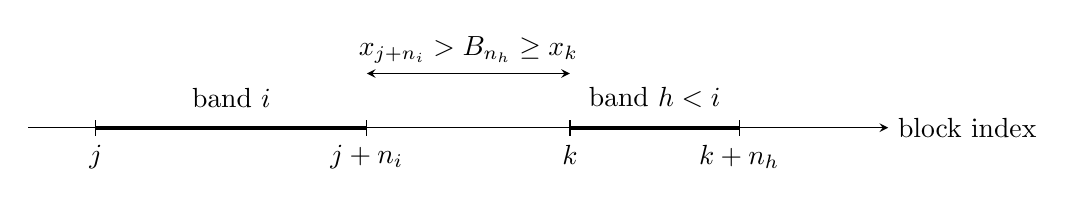
\begin{tikzpicture}[x=0.86cm,y=0.86cm,>=stealth]
 \draw[->] (0,0)--(12.7,0) node[right] {block index};
 \draw[line width=1.5pt] (1,0)--(5,0);
 \draw[line width=1.5pt] (8,0)--(10.5,0);
 \foreach \x in {1,5,8,10.5}{\draw (\x,-0.12)--(\x,0.12);}
 \node[below] at (1,-0.12) {$j$};
 \node[below] at (5,-0.12) {$j+n_i$};
 \node[below] at (8,-0.12) {$k$};
 \node[below] at (10.5,-0.12) {$k+n_h$};
 \node[above] at (3,0.15) {band $i$};
 \node[above] at (9.25,0.15) {band $h<i$};
 \draw[<->] (5,0.8)--(8,0.8);
 \node[above] at (6.5,0.8) {$x_{j+n_i}>B_{n_h}\ge x_k$};
\end{tikzpicture}
\caption{At a fixed target depth, a retained window from a finer band
ends before any retained window from a coarser band begins.  Here
$x_j=L-\lceil\sigma_j\rceil$ is nonincreasing in the block index.  The
schematic is not to scale.}
\label{fig:disjoint-windows}
\end{figure}

\subsection{Summing over target depths}

The disjointness lemma bounds the total gain at one physical scale.
Summing over targets recovers every pair scale in each band.  Indeed,
for a candidate $j\in J_i$,
\[
 0\le\sigma_j\le Dj\le T/2.
\]
Because $T$ is even, this also gives
$0\le\lceil\sigma_j\rceil\le T/2$.  Each integer
$\ell\in[a_{n_i},B_{n_i}]$ therefore occurs exactly once as
$L-\lceil\sigma_j\rceil$ for $1\le L\le T$: take
$L=\ell+\lceil\sigma_j\rceil$.  Its lower bound is $1$, and its
upper bound is at most $B_{n_i}+T/2<T$.

Each band has at least $T/(2Dn_i)$ candidate starts, and each contributes
expected pair mass at least $cn_i$ after summing the targets.  The block
length cancels, so every band supplies a fixed multiple of $T$.
Take expectations in \eqref{eq:telescoping-windows}.  Since the retention
indicator is $\mathcal F_{j+n_i}$-measurable, the tower property and
Lemma~\ref{lem:conditional-gain} apply to each summand.  Sum the result
over $L=1,\ldots,T$ and use the preceding exact correspondence to obtain
\begin{align}
 2T\log M
 &\ge\frac\delta2\sum_{i=1}^q\sum_{j\in J_i}
 \E\left[
 \mathbf1_{E_{n_i}}(\theta^j\omega)
 \sum_{\ell=a_{n_i}}^{B_{n_i}}
 c_\ell(\nu_{\theta^j\omega,n_i})\right]
 \notag\\
 &\ge\frac{\delta c}{2}\sum_{i=1}^q |J_i|n_i
 \ge\frac{\delta c qT}{4D}.
 \label{eq:final-window-count}
\end{align}
The second inequality uses Proposition~\ref{prop:pair-bands} and the
identical distribution of the type environment under $\theta^j$;
independence between different candidate windows is not needed.  The
last inequality follows from the exact count
\[
 |J_i|=\left\lfloor\frac{T}{2Dn_i}\right\rfloor+1
 \ge\frac{T}{2Dn_i}.
\]
After canceling $T$, \eqref{eq:final-window-count} bounds the arbitrary
integer $q$ by $8D\log M/(\delta c)$.  All the constants in this bound
were fixed before $q$ was chosen, so this is impossible.

\begin{proof}[Completion of the proof of Theorem~\ref{thm:main}]
The standard upper bound gives
$\dim_H\mu\le\min\{1,h/\chi\}$.  If the inequality were strict,
then $d=\dim_H\mu$ would satisfy $d<1$ and $d\chi<h$.
Section~\ref{sec:types} would supply the pair bands used above, and
\eqref{eq:final-window-count} would give a contradiction.  Therefore
$\dim_H\mu=\min\{1,h/\chi\}$ for the prescribed positive vector
$p$.  Since $p$ was arbitrary, the conclusion holds for every such
vector, including the cases $h=\chi$ and $h>\chi$.
\end{proof}

\section{Overlap conventions and dimension of the attractor}
\label{sec:corollaries}

We first reconcile the two usual word-length conventions for an exact overlap.
The following observation also appears in \cite[footnote~3]{Hochman2014}.
The nonzero contraction hypothesis is useful here as well as in the proof of
the measure theorem.

\begin{lemma}\label{lem:overlap-lengths}
For a finite family of maps $x\mapsto r_i x+t_i$ with $0<|r_i|<1$,
an equality of maps for two distinct nonempty words of arbitrary lengths
implies such an equality for two distinct words of the same length.
\end{lemma}
\begin{proof}
Suppose $\varphi_u=\varphi_v$ and $u\ne v$. If $u$ were a proper prefix
of $v$, writing $v=uw$ and cancelling the invertible map $\varphi_u$
would give $\varphi_w=\mathrm{id}$. This is impossible because a nonempty
word has absolute contraction less than one. The same applies with the
words interchanged. Now
$\varphi_{uv}=\varphi_u\circ\varphi_v
=\varphi_v\circ\varphi_u=\varphi_{vu}$.
The words $uv$ and $vu$ have the same length and are distinct: if they
were equal, their first $\min\{|u|,|v|\}$ symbols would show that either
$u=v$ or the shorter word is a proper prefix of the longer.
\end{proof}

\begin{corollary}[No exact overlaps]\label{cor:no-overlaps}
Let $\Phi$ be a finite nonempty indexed family of real similarities
with $0<|r_i|<1$ and no exact overlaps.  For every strictly positive
probability vector $p$,
\[
 \dim_H\mu_{\Phi,p}=\min\{1,H(p)/\chi(\Phi,p)\}.
\]
\end{corollary}
\begin{proof}
At every length $n$, distinct words give distinct complete maps.
Hence $G_n$ is an injective function of its symbol word, so
$H(G_n)=nH(p)$ and $h_{\mathrm{RW}}=H(p)$.
Apply Theorem~\ref{thm:main}.
\end{proof}

Let $K_\Phi$ be the compact attractor, equivalently the set of all coding
limits. Its similarity dimension $s_*$ is the unique number $s_*\ge0$
satisfying
\[
 \sum_{i\in\Lambda}|r_i|^{s_*}=1.
\]
For at least two symbols, existence and uniqueness follow because this sum
is continuous and strictly decreasing from $|\Lambda|>1$ to zero.
For one symbol its unique solution is zero.

\begin{corollary}\label{cor:set}
For a finite nonempty family of similarities of $\R$ with arbitrary real
translations and $0<|r_i|<1$, absence of exact overlaps implies
\[
 \dim_H K_\Phi=\min\{1,s_*\}.
\]
\end{corollary}
\begin{proof}
For one map the attractor is its fixed point and $s_*=0$.
For at least two maps choose the strictly positive weights
$p_i=|r_i|^{s_*}$. Then $H(p)=s_*\chi(\Phi,p)$.
Corollary~\ref{cor:no-overlaps} gives a measure supported on $K_\Phi$ of
dimension $\min\{1,s_*\}$, which is a lower bound for its set dimension.
For the upper bound, if $a>s_*$, the level-$n$ cylinder sets cover
$K_\Phi$, their diameters tend uniformly to zero, and
\[
 \sum_{u\in\Lambda^n}(\operatorname{diam}\varphi_u(K_\Phi))^a
 = (\operatorname{diam}K_\Phi)^a
   \left(\sum_i|r_i|^a\right)^n\longrightarrow0.
\]
The zero-diameter case is immediate. Thus $\dim_H K_\Phi\le s_*$,
and the ambient upper bound is one.
\end{proof}

\begin{corollary}\label{cor:homogeneous}
Let $m\ge2$, $0<\lambda<1$, and $t_1,\ldots,t_m\in\R$.
If the maps $x\mapsto\lambda x+t_i$ have no exact overlaps, then for
every strictly positive probability vector $p$ their self-similar measure has
\[
 \dim_H\mu=\min\left\{1,\frac{H(p)}{\log(1/\lambda)}\right\}.
\]
\end{corollary}
\begin{proof}
Apply Corollary~\ref{cor:no-overlaps} with $r_i=\lambda$ for every $i$.
Since the weights sum to one, $\chi=\log(1/\lambda)$.
\end{proof}

\begin{corollary}[Three maps]\label{cor:three-maps}
Let $0<\lambda<1$ and $t\in\R$.  If the indexed maps
\[
 x\longmapsto\lambda x,\qquad
 x\longmapsto\lambda x+1,\qquad
 x\longmapsto\lambda x+t
\]
have no exact overlaps, then for every $p_0,p_1,p_2>0$ with
$p_0+p_1+p_2=1$, their self-similar measure satisfies
\[
 \dim_H\mu
 =\min\left\{1,\frac{-\sum_{i=0}^2 p_i\log p_i}
                         {\log(1/\lambda)}\right\}.
\]
\end{corollary}
\begin{proof}
Apply Corollary~\ref{cor:homogeneous} with translations $0,1,t$.
\end{proof}

No claim of absolute continuity, effective separation, or a quantitative rate
of convergence follows from these dimension statements. In particular, the
finite upper endpoints of the scale ranges used in the proof have no asserted
effective bound.

\bibliographystyle{plain}
\bibliography{references}
\end{document}
